%
% nilpotent.tex
%
% (c) 2021 Prof Dr Andreas Müller, OST Ostschweizer Fachhochschule
%
\bgroup
\definecolor{darkgreen}{rgb}{0,0.6,0}
\def\feld#1{
	\fill[color=red!20] (#1,0) rectangle ({#1+1},12);
}
\begin{frame}[t]
\frametitle{$\mathcal{J}^k(f)$ und $\mathcal{K}^k(f)$ für nilpotente Matrizen}
\begin{columns}[t,onlytextwidth]
\begin{column}{0.42\textwidth}
Matrix mit dem dargestellten Verlauf von
${\color{red}\dim\mathcal{K}^k(A)}$
\begin{center}
\begin{tikzpicture}[>=latex,thick,scale=0.42]

\only<2->{
	\feld{0}
	\feld{1}
	\feld{2}
	\feld{3}
}
\only<2->{ \feld{4} }
\only<2->{ \feld{6} }
\ifthenelse{\boolean{presentation}}{
\only<3->{ \feld{5} }
\only<3->{ \feld{7} }
\only<4->{ \feld{8} }
\only<5->{ \feld{9} }
\only<6->{ \feld{10} }
\only<7->{ \feld{11} }

\only<1>{ \node at (6,0) [below] {$k=0$}; }
}{}
\only<2>{ \node at (6,0) [below] {$k=1$}; }
\ifthenelse{\boolean{presentation}}{
\only<3>{ \node at (6,0) [below] {$k=2$}; }
\only<4>{ \node at (6,0) [below] {$k=3$}; }
\only<5>{ \node at (6,0) [below] {$k=4$}; }
\only<6>{ \node at (6,0) [below] {$k=5$}; }
\only<7>{ \node at (6,0) [below] {$k=6$}; }
}{}

\draw (0,0) rectangle (12,12);
\ifthenelse{\boolean{presentation}}{
\only<1>{
	\foreach \x in {1,...,12}{
		\node at ({\x-0.5},{12-\x+0.5}) {$1$};
	}
}
}{}
\only<2->{
	\foreach \x in {1,...,12}{
		\node at ({\x-0.5},{12-\x+0.5}) {$0$};
	}
}
\only<2>{
	\foreach \x in {7,...,11}{
		\node at ({\x+0.5},{12-\x+0.5}) {$1$};
	}
}
\ifthenelse{\boolean{presentation}}{
\only<3->{
	\foreach \x in {7,...,11}{
		\node at ({\x+0.5},{12-\x+0.5}) {$0$};
	}
}
\only<3>{
	\foreach \x in {8,...,11}{
		\node at ({\x+0.5},{13-\x+0.5}) {$1$};
	}
}
\only<4->{
	\foreach \x in {8,...,11}{
		\node at ({\x+0.5},{13-\x+0.5}) {$0$};
	}
}
\only<4>{
	\foreach \x in {9,...,11}{
		\node at ({\x+0.5},{14-\x+0.5}) {$1$};
	}
}
\only<5->{
	\foreach \x in {9,...,11}{
		\node at ({\x+0.5},{14-\x+0.5}) {$0$};
	}
}
\only<5>{
	\foreach \x in {10,...,11}{
		\node at ({\x+0.5},{15-\x+0.5}) {$1$};
	}
}
\only<6->{
	\foreach \x in {10,...,11}{
		\node at ({\x+0.5},{15-\x+0.5}) {$0$};
	}
}
\only<6>{
	\foreach \x in {11,...,11}{
		\node at ({\x+0.5},{16-\x+0.5}) {$1$};
	}
}
\only<7->{
	\foreach \x in {11,...,11}{
		\node at ({\x+0.5},{16-\x+0.5}) {$0$};
	}
}
}{}
\draw[line width=0.1pt]
	(0,11) -- (2,11) -- (2,9) -- (4,9) -- (4,6) -- (12,6);
\draw[line width=0.1pt]
	(1,12) -- (1,10) -- (3,10) -- (3,8) -- (6,8) -- (6,0);
\only<2>{
	\node at (5.5,7.5) {$1$};
}
\ifthenelse{\boolean{presentation}}{
\only<3->{
	\node at (5.5,7.5) {$0$};
}
}{}
\end{tikzpicture}
\end{center}
\end{column}
\begin{column}{0.56\textwidth}
\vspace{-15pt}
\begin{center}
\begin{tikzpicture}[>=latex,thick]
\def\pfad{
	(0,0) -- (1,3) -- (2,4) -- (3,4.5) -- (4,5) -- (5,5.5) -- (6,6)
}
\fill[color=orange!20] \pfad -- (0,6) -- cycle;
\fill[color=darkgreen!20] \pfad -- (6,0) -- cycle;
\foreach \y in {0.5,1,...,5.75}{
	\draw[line width=0.1pt] (0,\y) -- (6,\y);
}
\draw[line width=1.4pt] \pfad;
\draw[->] (-0.1,6) -- (6.5,6); \node at (-0.1,6) [left] {$n$};
\draw[->] (-0.1,0) -- (6.5,0); \node at (-0.1,0) [left] {$0$};
\fill (0,0) circle[radius=0.05];
\fill (1,3) circle[radius=0.05];
\fill (2,4) circle[radius=0.05];
\fill (3,4.5) circle[radius=0.05];
\fill (4,5) circle[radius=0.05];
\fill (5,5.5) circle[radius=0.05];
\fill (6,6) circle[radius=0.05];
\ifthenelse{\boolean{presentation}}{
\only<1>{
	\fill[color=red] (0,0) circle[radius=0.08];
}
}{}
\only<2>{
	\fill[color=red] (1,3) circle[radius=0.08];
	\draw[color=red] (0,3) -- (1,3);
	\node[color=red] at (0,3) [left] {$6$};
}
\ifthenelse{\boolean{presentation}}{
\only<3>{
	\fill[color=red] (2,4) circle[radius=0.08];
	\draw[color=red] (0,4) -- (2,4);
	\node[color=red] at (0,4) [left] {$8$};
}
\only<4>{
	\fill[color=red] (3,4.5) circle[radius=0.08];
	\draw[color=red] (0,4.5) -- (3,4.5);
	\node[color=red] at (0,4.5) [left] {$9$};
}
\only<5>{
	\fill[color=red] (4,5.0) circle[radius=0.08];
	\draw[color=red] (0,5.0) -- (4,5.0);
	\node[color=red] at (0,5.0) [left] {$10$};
}
\only<6>{
	\fill[color=red] (5,5.5) circle[radius=0.08];
	\draw[color=red] (0,5.5) -- (5,5.5);
	\node[color=red] at (0,5.5) [left] {$11$};
}
\only<7>{
	\fill[color=red] (6,6.0) circle[radius=0.08];
}
}{}
\draw[color=white] (-0.7,0) -- (-0.7,6);
\end{tikzpicture}
\end{center}
\end{column}
\end{columns}
\end{frame}
\egroup
